%\documentclass{beamer} 
\documentclass[handout]{beamer} 
\usetheme{Ilmenau}
\usepackage{graphicx,verbatim,hyperref}
\usepackage{textpos}

\usecolortheme{beaver}
\useinnertheme{default}
\setbeamertemplate{itemize item}[triangle]
\setbeamertemplate{itemize subitem}[triangle]
\setbeamertemplate{itemize subsubitem}[circle]
\setbeamertemplate{enumerate items}[default]
\setbeamertemplate{blocks}[upper=block head,rounded]
\setbeamercolor{item}{fg=black}
\usefonttheme{serif} %should allow ccfonts to take effect

\usepackage{cite}
\usepackage{xcolor,bm}
\usepackage{amsbsy,amssymb, amsmath, amsthm}
\usepackage{booktabs}
%David miller's fonts
	\usepackage[T1]{fontenc}
	\usepackage[boldsans]{ccfonts}
	\usepackage[euler-hat-accent]{eulervm}

\newcommand{\al}{\alpha}
\newcommand{\expect}{\mathbb{E}}
\newcommand{\Bt}{B(\bm{\tau^a})}
\newcommand{\bta}{\bm{\tau^a}}
\newcommand{\btn}{\bm{\tau^{tw}}}
\newcommand{\ga}{\gamma}
\newcommand{\ve}{\varepsilon}
\newcommand{\ta}{\theta}

\newenvironment{changemargin}[2]{% 
  \begin{list}{}{% 
    \setlength{\topsep}{0pt}% 
    \setlength{\leftmargin}{#1}% 
    \setlength{\rightmargin}{#2}% 
    \setlength{\listparindent}{\parindent}% 
    \setlength{\itemindent}{\parindent}% 
    \setlength{\parsep}{\parskip}% 
  }% 
  \item[]}{\end{list}} 
	
	\let\Tiny=\tiny


\title[Explaining Gradualism in Trade Liberalization \hspace{2.5in}\insertframenumber/\inserttotalframenumber]{Explaining Gradualism in Trade Liberalization: \\A Political Economy Approach}
\author[Kristy Buzard]{\texorpdfstring{Kristy Buzard\newline Syracuse University  \newline\url{kbuzard@syr.edu}}{Kristy Buzard}}
\date{May 17, 2017}

\begin{document}
\maketitle
%\insertpresentationendpage removed b/c of appendix




\section{Overview}
\subsection{Preview}

\begin{frame}{Average tariffs for U.S., Western Europe, and Japan}
	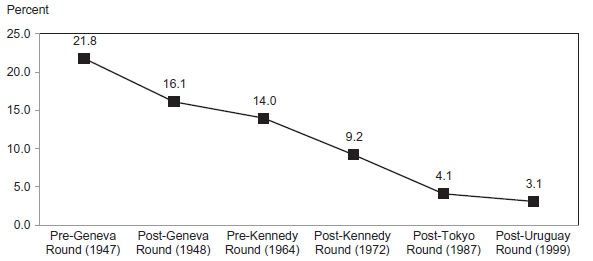
\includegraphics[height=2in, width=4.25in]{linegraph-Bown-Irwin.png} \\
	\scriptsize Source: Bown, C.P., Irwin, D.A., (2017) ``The GATT's Starting Point: Tariff Levels circa 1947,'' in Assessing the World Trade Organization: Fit for Purpose?, M. Elsig, B. Hoekman, and J. Pauwelyn eds., Cambridge University Press, forthcoming, fig. 1
	%based on backcast estimates for 1947 average tariffs, computed from data on simple average tariffs in effect at the beginning of the Kennedy Round (1964), and reports on the size of average tariff cuts arising during the initial GATT negotiating rounds.
\end{frame}

\begin{frame}
\frametitle{The Questions}
\pause
\begin{enumerate}[<+->]
	\item Why would liberization not be immediate? Why proceed in stages?
  \item What are the frictions preventing free trade? %assuming free trade is efficient
\end{enumerate}
\end{frame}



\begin{frame}
\frametitle{Related Literature}

Export sector
\begin{itemize}
  \item \footnotesize Benefits of trade integration to consumers (Devereau 1997)
  \item \footnotesize Exporters increasingly dependent on trade via capacity accumulation (Chisik 2003)
\end{itemize}

\vskip.1in
Import-competing sector
\begin{itemize}
  \item \footnotesize Convex adjustment costs as workers leave import-competing sector (Mussa 1986); Furusawa $\&$ Lai similar for repeated game
	\item \footnotesize Gradual reductions improve welfare when there's a minimum wage (Mehlum 1998)
	\item \footnotesize Workers lose specialized skills as they leave (Staiger 1995)
\end{itemize}

Limitation of punishments to `withdrawal of equivalent concessions' generates gradualism (Zissimos 2007)

\begin{itemize}
	\item MRC?
\end{itemize}

\end{frame}


\begin{frame}
\frametitle{Politics: Motivation}

Is there a \textit{fundamentally} political economy explanation for gradualism?
\begin{itemize}
	\item i.e. a story that doesn't hinge on specific nature of trade
	\item The hope: lessons could be applied to other issue areas
\end{itemize}

\end{frame}


\begin{frame}
\frametitle{Politics: Mechanism}

Inefficient tariffs maintained through the lobbying of import-competing industries
\begin{itemize}
	\item BUT ability to maintain protection reduced by shocks to political support
		\begin{itemize}
			\item a key politician losing an election or committee position
		\end{itemize}
	\item Immediate loss of protection / rents \textit{can} $\Rightarrow$ erosion of future political power and accompanying protection
	\item Demonstrate with a dynamic model of political economy
\end{itemize}

\end{frame}

\begin{comment}
\begin{frame}{Institutional Detail}
\begin{itemize}[<+->]
	\item  
		\begin{itemize}
			\item  
			\item  
		\end{itemize}
	\item 
	\item 
		\begin{itemize}
			\item  
		\end{itemize}
	\item  
		\begin{itemize}
			\item  
			\item  
		\end{itemize}
\end{itemize}
\end{frame}
\end{comment}
 
\begin{frame}{Preview of Results}

\pause
The 
\pause
\begin{itemize}[<+->]
	\item I
	\item D
	\item I
\end{itemize}
\end{frame}





\section{Model}
\subsection{Economic and Political Structure}
\begin{frame}{Timeline}
\pause

Taking trade agreement tariff and anti-dumping duties as given,
\pause
\begin{enumerate}[<+->]
	\item \textbf{Import-competing firms lobby DOC/ITC to renew AD duties}
	\item \textbf{Uncertainty is resolved}
	\item \textbf{DOC/ITC decide whether to renew duties}
	\item Private actors make production, consumption decisions
\end{enumerate}
\end{frame}


\begin{frame}{Economy}
\begin{itemize}
	\item Two countries: home and foreign (${}^*$)
	\item Separable in three goods: $X$ and $Y$ (traded) and numeraire
	\item Demand identical for both goods in both countries
	\item Supply: $Q_X^*(P_X) > Q_X(P_X)$ $\forall P_X$; symmetric for $Y$ 
		\begin{itemize}
			\item Home net importer of $X$, net exporter of $Y$
		\end{itemize}
\end{itemize}

\vskip.2in
\pause
Home levies $\tau$ on $X$, Foreign levies $\tau^*$ on $Y$
\pause
\begin{itemize}
	\item $P_X=P_X^W + \tau$ and $\pi_X(P_X)$ increasing in $\tau$
\end{itemize}

\pause
\vskip.2in
Non-tradable specific factors motivates political activity


\end{frame}


\begin{frame}{Political Structure}
In Home country (foreign is passive):
\pause
\begin{itemize}[<+->]
	\item Dept. of Commerce 
		\begin{itemize}[<+->]
			\item Can 
			\item Susceptible 
			\item Modeled 
		\end{itemize}
%\pause
	\item A Single Lobby
		\begin{itemize}
			\item Represents import-competing sector, $X$
		\end{itemize}	
\end{itemize}

\end{frame}


\subsection{The Players}
\begin{frame}
\frametitle{``Government''}
\pause
Decision determined by complex process. Reduced form:
\pause
\[
  W_G = \mathit{CS}_X(\tau) + \ga(e,\ta) \pi_X(\tau) + \mathit{CS}_Y(\tau^*) + \pi_Y(\tau^*) + \mathit{TR}(\tau)
\]

\pause
\begin{itemize}[<+->]
	\item $\mathit{CS_i(\cdot)}$: consumer surplus
	\item $\pi_X(\tau)$: profits of import-competing industry
	\item $\pi_Y(\tau^*)$: profits of exporting industry
	\item $\mathit{TR}(\tau)$: tariff revenue
\end{itemize}
\end{frame}


\begin{frame}
\frametitle{``Government''}
\[
  W_G = \mathit{CS}_X(\tau) + \ga(e,\ta) \pi_X(\tau) + \mathit{CS}_Y(\tau^*) + \pi_Y(\tau^*) + \mathit{TR}(\tau)
\]

\pause
\begin{itemize}
	\item $\ga(e,\ta)$: weight on import-competing industry profits
		\begin{itemize}
			\pause
			\item $e$: lobbying effort
			\pause
			\item $\ta$: uncertain element in $G$'s preferences
		\end{itemize}
\end{itemize}

\pause
\vskip.1in
\begin{beamerboxesrounded}[upper=palette tertiary, shadow=true]{Assumption 1}
\begin{enumerate}
  \pause
	\item $\ga(e,\ta)$ is increasing and concave in $e$ for all $\ta \in \Theta$.
\end{enumerate}
\end{beamerboxesrounded}
\end{frame}


\begin{frame}
\frametitle{Lobby}
\vskip.2in
\pause
Lobby chooses effort to maximize:
\[
  \left\{1-\Pr\left[ \text{AD Renewal}\right]\right\} \ \pi(\tau^a) + \Pr\left[ \text{AD Renewal} \right]  \pi(\tau^{\mathit{ad}})  - e
\]

\vskip.1in
\pause
\begin{itemize}[<+->]
	\item $e$: Lobbying effort
	\item $\tau^a$: home import tariff under trade agreement
	\item $\tau^{\textit{ad}}$: home import tariff equivalent under anti-dumping duties
\end{itemize}

\vskip.1in
Note: In Staiger (1995), gradualism breaks down in workers can organize

\end{frame}


\section{Uncertainty}
\subsection{}
\begin{frame}{Timeline}
\begin{enumerate}[<+->]
	\item \textbf{Import-competing firms lobby ...}
	\item {\color{gray} \textbf{Uncertainty is resolved}}
	\item \textbf{Government ...}
	\item {\color{gray} Private actors make production, consumption decisions}
\end{enumerate}
	
\end{frame}

\begin{frame}{Why uncertainty?}
\pause
\textbf{Government}
\pause
\begin{itemize}
	\item Renews AD duties if $G$ prefers $\tau^{\mathit{ad}}$ to $\tau^a$
\end{itemize}

\pause
\vskip.1in
\textbf{Lobby}
\pause
\begin{itemize}[<+->]
	\item Given $(\tau^a,\tau^{*a})$ and $\tau^{\mathit{ad}}$, lobby knows what $e$ is required to induce renewal
 	\item Lobby pays this $e$ if: \hskip.2in $\pi(\tau^{\mathit{ad}}) - e > \pi(\tau^a)$
\end{itemize}

\pause
\vskip.1in
\textbf{In Equilibrium}
\pause
\begin{itemize}[<+->]
	\item Firms only put forth effort when they know renewal will be granted
\end{itemize}

\end{frame}


\begin{frame}{What's this uncertainty about?}
\pause
Lobby  
\begin{itemize}[<+->]
	\item But
	\item But
\end{itemize}

\pause
\vskip.1in
So what's the uncertainty about?
\pause
\begin{itemize}[<+->]
	\item Probability foreign will retaliate or initiate dispute (indirect)
	\item $G$'s valuation of harm to industry, e.g. how politically important is industry?
\end{itemize}

\end{frame}


\section{Results}
\subsection{}
\begin{frame}{Timeline}
\begin{enumerate}[<+->]
	\item \textbf{Import-competing firms lobby DOC/ITC to renew AD duties}
	\item \textbf{Uncertainty is resolved}
	\item \textbf{DOC/ITC decide whether to renew duties}
	\item Private actors make production, consumption decisions
\end{enumerate}
\end{frame}


\begin{frame}{Government}
  $G$ renews AD duties if its utility is higher under AD duties than trade agreement tariff
	\pause
  \begin{itemize}
		\item Preferences are ex-ante uncertain through $\ta$
		\pause
		\item When does $G$ renew AD duties? \\
	\pause
  \vskip.1in
    $b(e,\tau^a,\tau^{\textit{ad}})$: probability $G$ prefers $\tau^{ad}$ to $\tau^a$ for a given effort level $e$
\end{itemize}

\pause
\vskip.25in
\begin{beamerboxesrounded}[upper=palette tertiary, shadow=true]{Lemma 1}
  The probability that $G$ renews AD duties is increasing and concave in lobbying effort $e$ $\left(\text{i.e. } \frac{\partial b}{\partial e} \geq 0, \ \frac{\partial^2 b}{\partial e^2} \leq 0  \right)$.
\end{beamerboxesrounded}

\end{frame}

\begin{frame}{Home's Trade Agreement Tariff}

\pause
\begin{beamerboxesrounded}[upper=palette tertiary, shadow=true]{Result 1}
  The total probability that $G$ renews AD duties is decreasing in the home trade agreement tariff $\tau^a$.
\end{beamerboxesrounded}

\vskip.25in
\pause
There's both a direct effect and an indirect effect through lobby's incentives, and both are negative:
\[
  \frac{\partial b}{\partial e} \frac{\partial e}{\partial \tau^a} + \frac{\partial b}{\partial \tau^a}
\]
\end{frame}

\begin{frame}{Foreign's Trade Agreement Tariff}

Assuming trading partner does not retaliate
\pause
\begin{itemize}
	\item No difference in foreign tariff under AD duty and $\tau^a$. So no effect on $G$'s incentives (either direct or indirect)
\end{itemize}


\vskip.25in
\pause
\begin{beamerboxesrounded}[upper=palette tertiary, shadow=true]{Result 2}
  The total probability that $G$ renews AD duties is unaffected by foreign's trade agreement tariff $\tau^a$.
\end{beamerboxesrounded}
\end{frame}


\begin{frame}{Profitability of Import-Competing Sector}

\pause
\textit{NOTE: this is not quite right, but some version of it will be} \\
Assume $\pi(\cdot)$ shifts up uniformly for all $\tau$.
\pause
\begin{itemize}[<+->]
	\item Convexity of profits $\Rightarrow$ $G$'s marginal benefit of providing protection goes up
	\item Convexity of profits $\Rightarrow$ return from lobbying increases
\end{itemize}


\vskip.25in
\pause
\begin{beamerboxesrounded}[upper=palette tertiary, shadow=true]{Result 3}
  The total probability that $G$ renews AD duties is increasing in the profitability of the import-competing sector.
\end{beamerboxesrounded}
\end{frame}


\begin{frame}{Exogenous Shifts in $\ga(e,\ta)$}

\pause
Assume $\ga(\cdot,\cdot)$ shifts up uniformly for all $(e,\ta)$ pairs.
\pause
\begin{itemize}[<+->]
	\item $G$ gives more weight to firms' benefit
	\item Lobbying incentives are unchanged
\end{itemize}

\vskip.25in
\pause
\begin{beamerboxesrounded}[upper=palette tertiary, shadow=true]{Result 3}
  The total probability that $G$ renews AD duties increases when the weighting function shifts up exogenously and uniformly.
\end{beamerboxesrounded}
\end{frame}


\begin{frame}{Protection from AD Duties}

\pause
When $\tau^{\textit{ad}}$ increases, two effects on $G$'s incentives:
\pause
\begin{itemize}[<+->]
	\item Social welfare decreases, pushes for decrease in renewal probability 
	\item (Over-weighted) import-competing profits increase, pushes for increase in renewal probability 
\end{itemize}

\vskip.2in
\pause
Indirect effect is of same sign as direct effect
\pause
\begin{itemize}[<+->]
	\item When $\tau^{\textit{ad}}$ (i.e. close to social optimum), second effect dominates $\Rightarrow$ increase in renewal probability
	\item Effect may be concave
\end{itemize}

\end{frame}


\section{Conclusion}
\subsection{}
\begin{frame}{Future Work}
\pause
\begin{itemize}[<+->]
	\item Comparative static 
	\item Empirical 
	\item Extend model 
\end{itemize}
\end{frame}


\end{document}